\documentclass{beamer}

\title{Section 2}
\author{TA: Dante Buhl}
\institute{UCSC Math-19B}
%\date{Week 2}
\graphicspath{ {./images/} }
%\usepackage{xcolor}
\usepackage{verbatim}
\usetheme{Goettingen}
\usecolortheme{seahorse}
\usefonttheme{serif}
%\usepackage[x11names]{xcolor}
\usepackage{amsmath}
\usepackage{pifont}


\begin{document}

\newcommand{\bmp}[1]{\begin{minipage}{#1\textwidth}}
\newcommand{\emp}{\end{minipage}}


%Title
\frame{\titlepage}

\section{Welcome to Section!}
\begin{frame}{Plan for Today}
    Topics to Cover
    \begin{itemize}
        \item Review Activity
        \item Substitution Method
    \end{itemize}
    Section Activity 2
    \begin{itemize}
        \item 3 questions
    \end{itemize}
    Assignments
    \begin{itemize}
        \item Homework 2 (Due Fri, Jan. $26^{th}$)
    \end{itemize}
\end{frame}

\begin{frame}{Week 2 Reflections}
    
    \vspace{10pt}

    \bmp{.4}
       
    \emp
    \hspace{5pt}
    \bmp{.55}
        \centering
        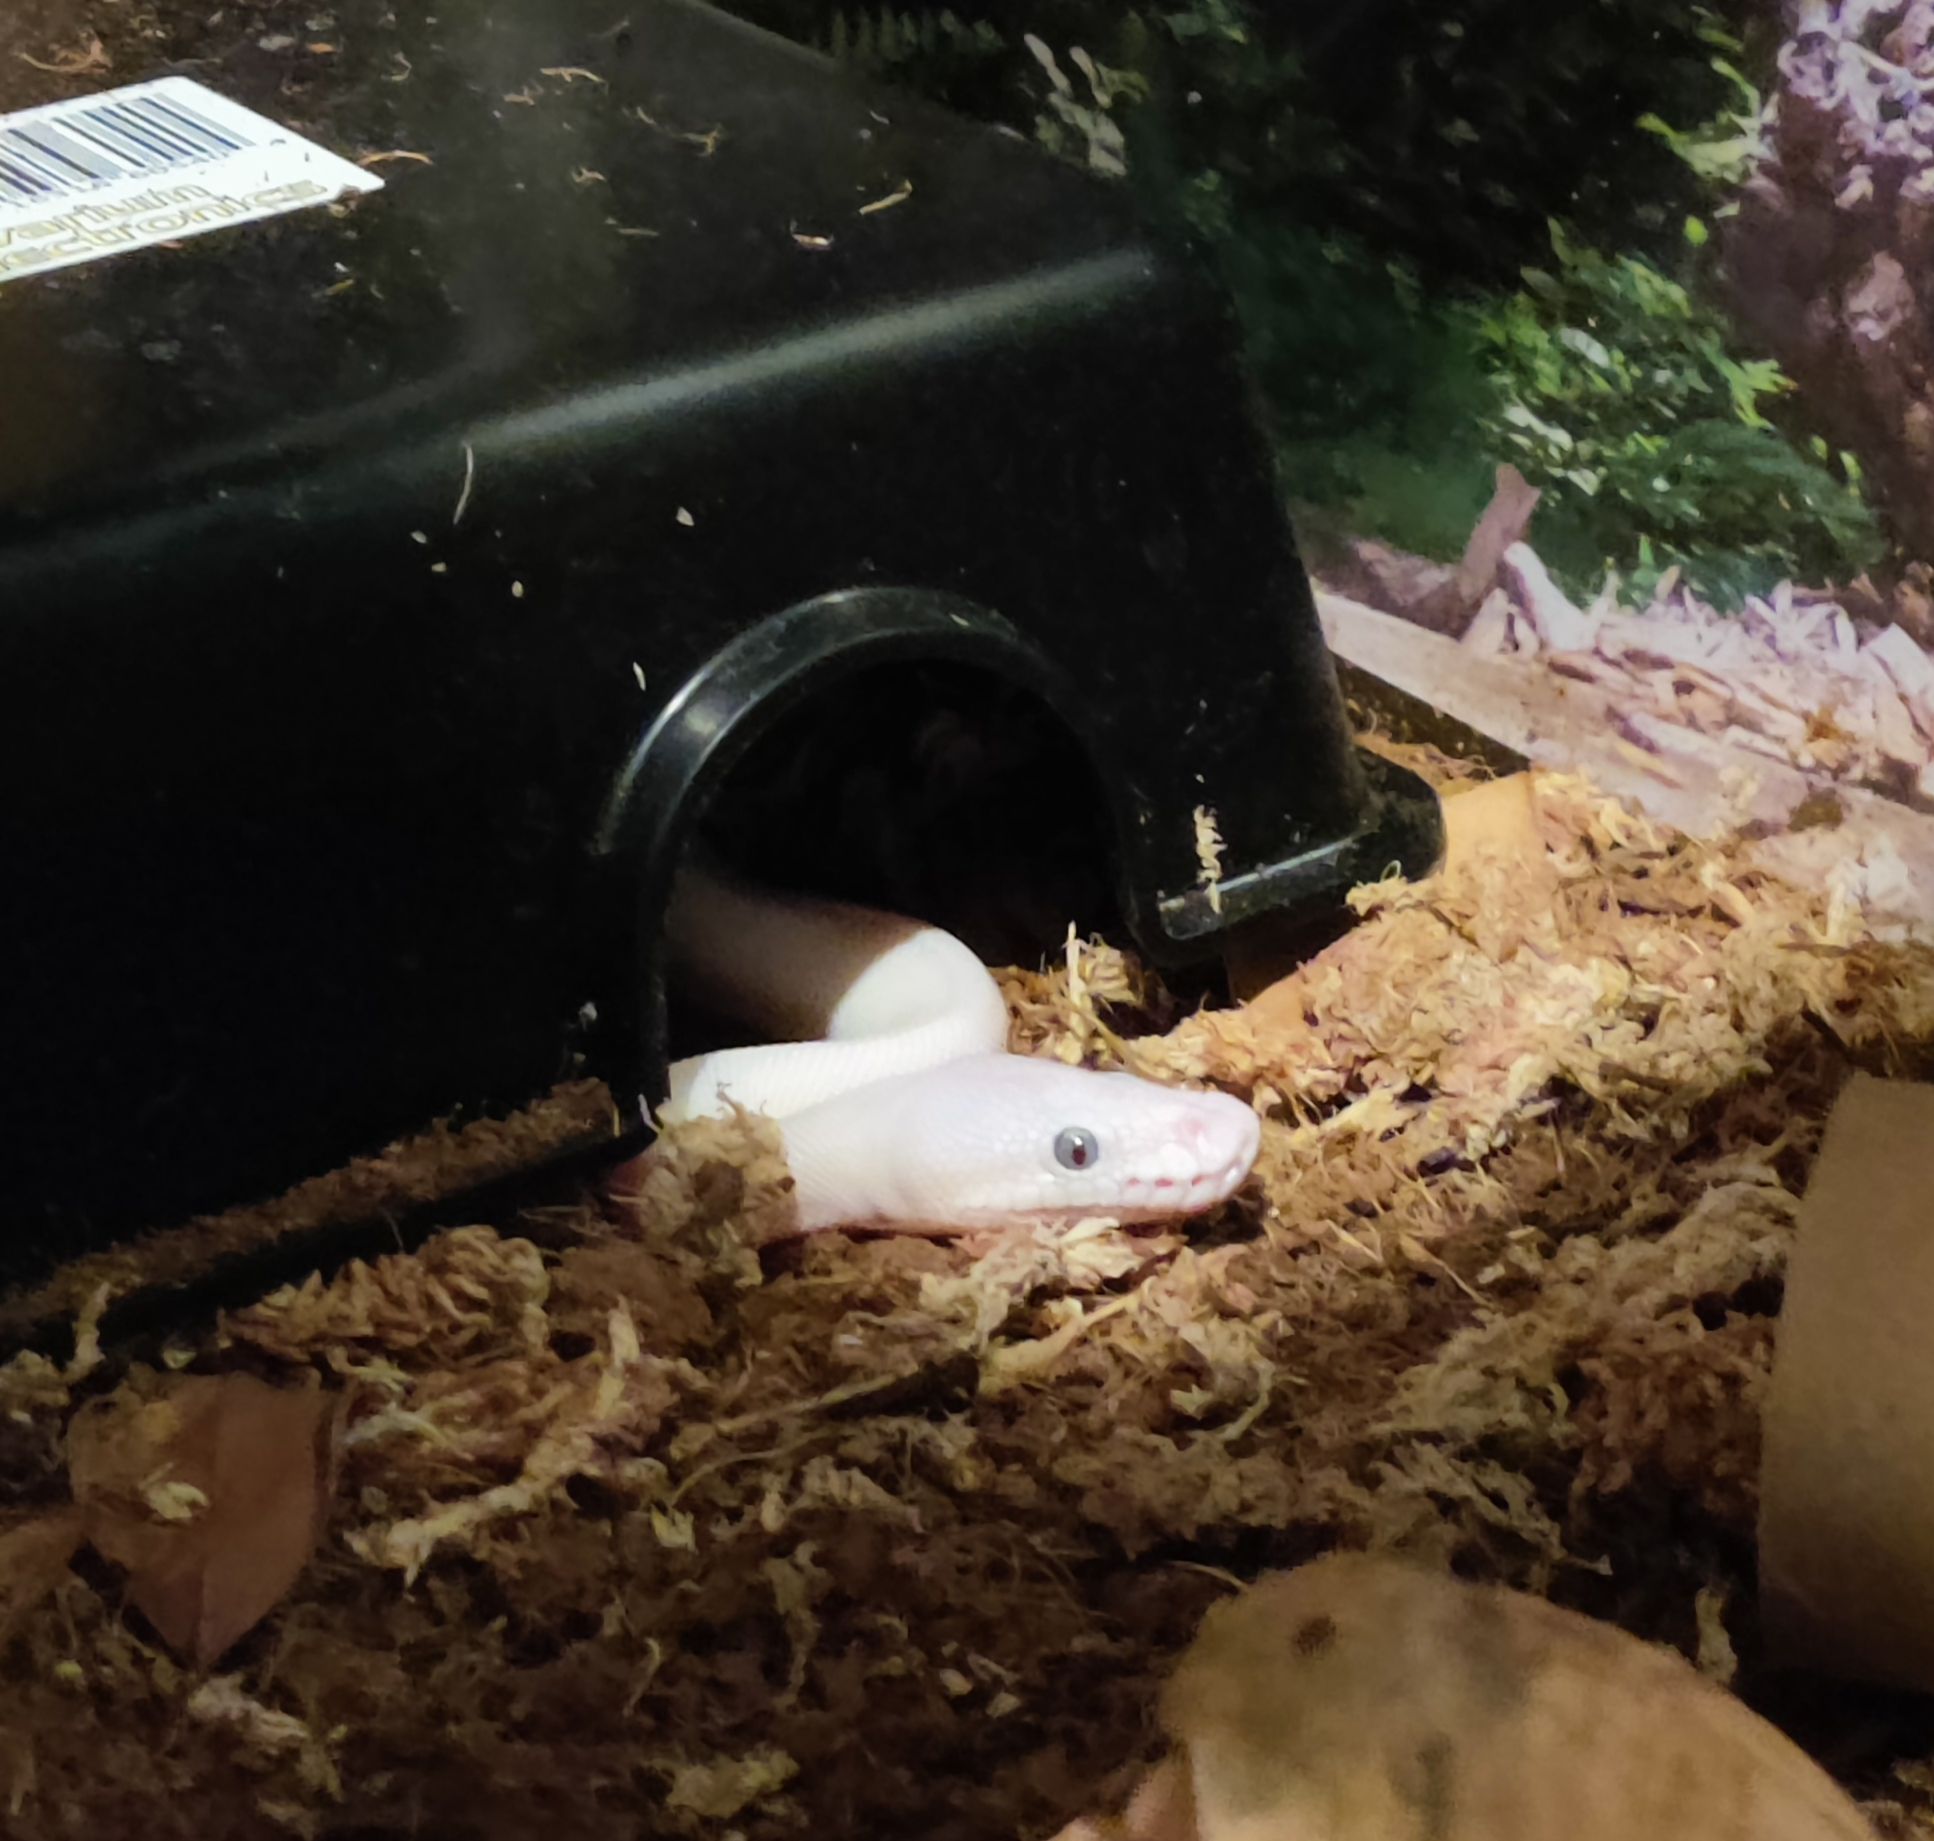
\includegraphics[width=.75\textwidth]{duncan.jpg}
    \emp
\end{frame}


\begin{frame}{Learning Outcomes}
    \begin{itemize}
        \item Using FTC P.1 and P.2 to compute integrals.
        \item Develop strategies for finding anti-derivatives.
        \item Understand how to use and apply u-substitution for integrals/anti-derivatives.
    \end{itemize}
\end{frame}

\section{Practice}
\begin{frame}{Review Activity}

    
\includegraphics[width=.6\textwidth]{activity.png}


\end{frame}


\begin{frame}{Section Activity 2 (Access Code: )}
    
\end{frame}

\end{document}
